\section{Numerical solution using a collocation BVP solver}
\subsection{Problem}
We solve the coupled ODE system on \(z\in[0,\infty)\):
\[
\begin{aligned}
v''(z) &= a(z)\,u(z),\\[4pt]
u''(z) &= -a(z)\,v(z),
\end{aligned}
\]
with boundary conditions at the surface
\[
v(0)=0,\qquad u(0)=-u_0,
\]
and the physical requirement
\[
u(z)\to 0,\quad v(z)\to 0 \quad (z\to\infty).
\]

\subsection{The idea}
\begin{enumerate}
  \item Replace the infinite domain by a large finite height \(z_{\max}\).
  \item At \(z_{\max}\) introduce a \emph{decay condition} that goes to zero rather than forcing exact zeros there.
  \item Convert the two second-order ODEs into a first-order system and solve the resulting boundary-value problem numerically (using a collocation BVP solver).
\end{enumerate}

\subsection{Why not force \(u=v=0\) at \(z_{\max}\)?}
Forcing \(u(z_{\max})=v(z_{\max})=0\) at a finite depth often gives error in that the solution does not go the zero slowly, and the solver might increase afterwards ( for example by oscillation). 

\subsection{Robin boundary condition}
If a function \(y(z)\) decays like \(y\!\propto\!e^{-k z}\) for large \(z\), then
\[
y'(z) = -k\,y(z) \quad \Longrightarrow \quad y'(z)+k\,y(z)=0.
\]
This is a first-order mixed Robin condition. For our system we know that we enter a region where $a=$constant, thus the solution becomes the classical Ekman spiral:
\begin{equation}
    \begin{cases}
        v''(z) = a u(z), \\
        u''(z) = -a v(z)
    \end{cases} \implies
    \begin{cases}
        u(z) = -u_0\exp(-k z)\cos(k z), \\
        v(z) = u_0\exp(-k z)\sin(k z),
    \end{cases}
\end{equation}
Where \(k=\sqrt{a/2}\). Taking the derrivative we obtain 
\begin{equation*}
    u'=-k(u-v),\quad
    v'= -k(u+v).
\end{equation*}
Thus at \(z=z_{\max}\) we impose the boundary conditions
\[
u'(z_{\max}) + k\,u(z_{\max}) - k\,v(z_{\max}) = 0,\qquad
v'(z_{\max}) + k\,u(z_{\max}) + k\,v(z_{\max}) = 0.
\]
Thus these new boundary conditions force the solver to choose solutions whose slope at high altitudes matches a decay rate \(k\). 

\subsection{How to choose the decay rate}
\begin{itemize}
  \item If \(a(z)=a_0\) is constant, then we get a  decay rate of \(k=\sqrt{a_0/2}\).
  \item If \(a(z)\) varies, one must use the limit of 
  of $k$ at the upper limit as $ k= \sqrt{a_{z_\text{max}}}/2$.
\end{itemize}

\subsection{Rewrite as a first-order system}
Define
\begin{equation}
Y(z) = \begin{bmatrix} u \\ u' \\ v \\ v' \end{bmatrix}.
\end{equation}
Then the ODEs become
\begin{equation}
Y' = \begin{bmatrix}
u' \\ -a(z)\,v \\ v' \\ a(z)\,u
\end{bmatrix}.
\end{equation}
We now have a first-order system \(Y' = F(z,Y)\) and four boundary conditions.
\begin{equation}
    \begin{cases}
    v(0)=0,\\[2pt]
    u(0)=-u_0,\\[2pt]
    u'(z_{\max}) + k\,u(z_{\max}) - k\,v(z_{\max}) = 0,\\[2pt]
v'(z_{\max}) + k\,u(z_{\max}) + k\,v(z_{\max}) = 0.
    \end{cases}
\end{equation}


\subsection{How the numerical solver (\texttt{solve\_bvp}) works}
Newton's method (or a Newton-like iteration) is used to solve that algebraic system. This requires an initial guess for the full solution profile. We use 
\begin{equation}
    u\sim-u_0 e^{-kz}\cos(kz), \
    v\sim u_0 e^{-kz}\sin(kz).
\end{equation}
the solver returns a polynomial solution.


\begin{figure}[H]
    \centering    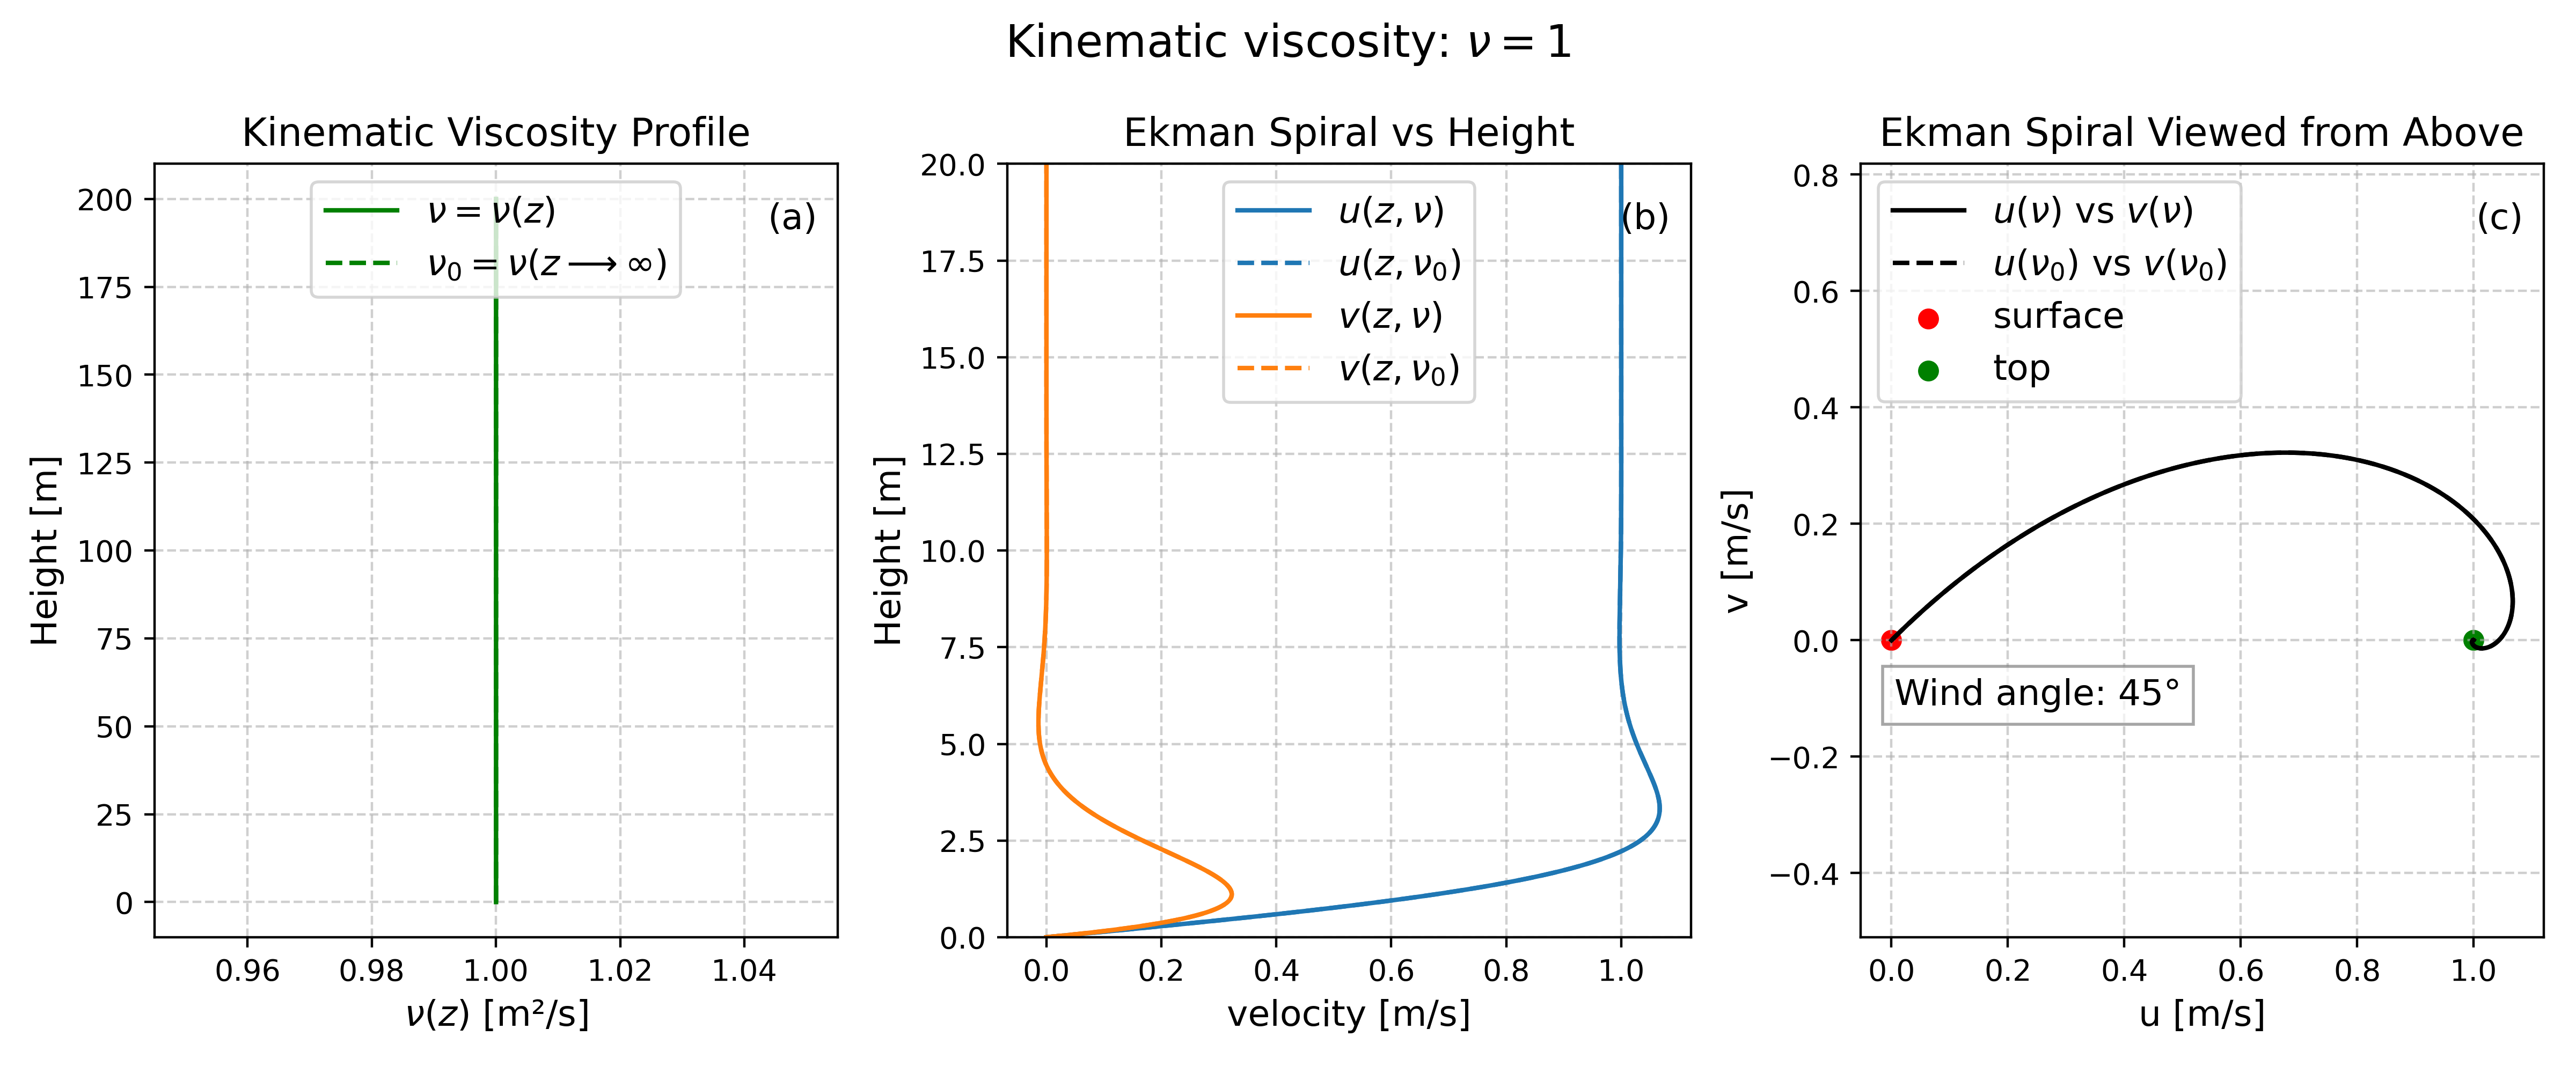
\includegraphics[width=0.9\textwidth]{Figures/BVP_const.png}
    \caption{This figure shows the numeric solution for an constant profile.}
    \label{fig:numeric_const}
\end{figure}

\begin{figure}[H]
    \centering    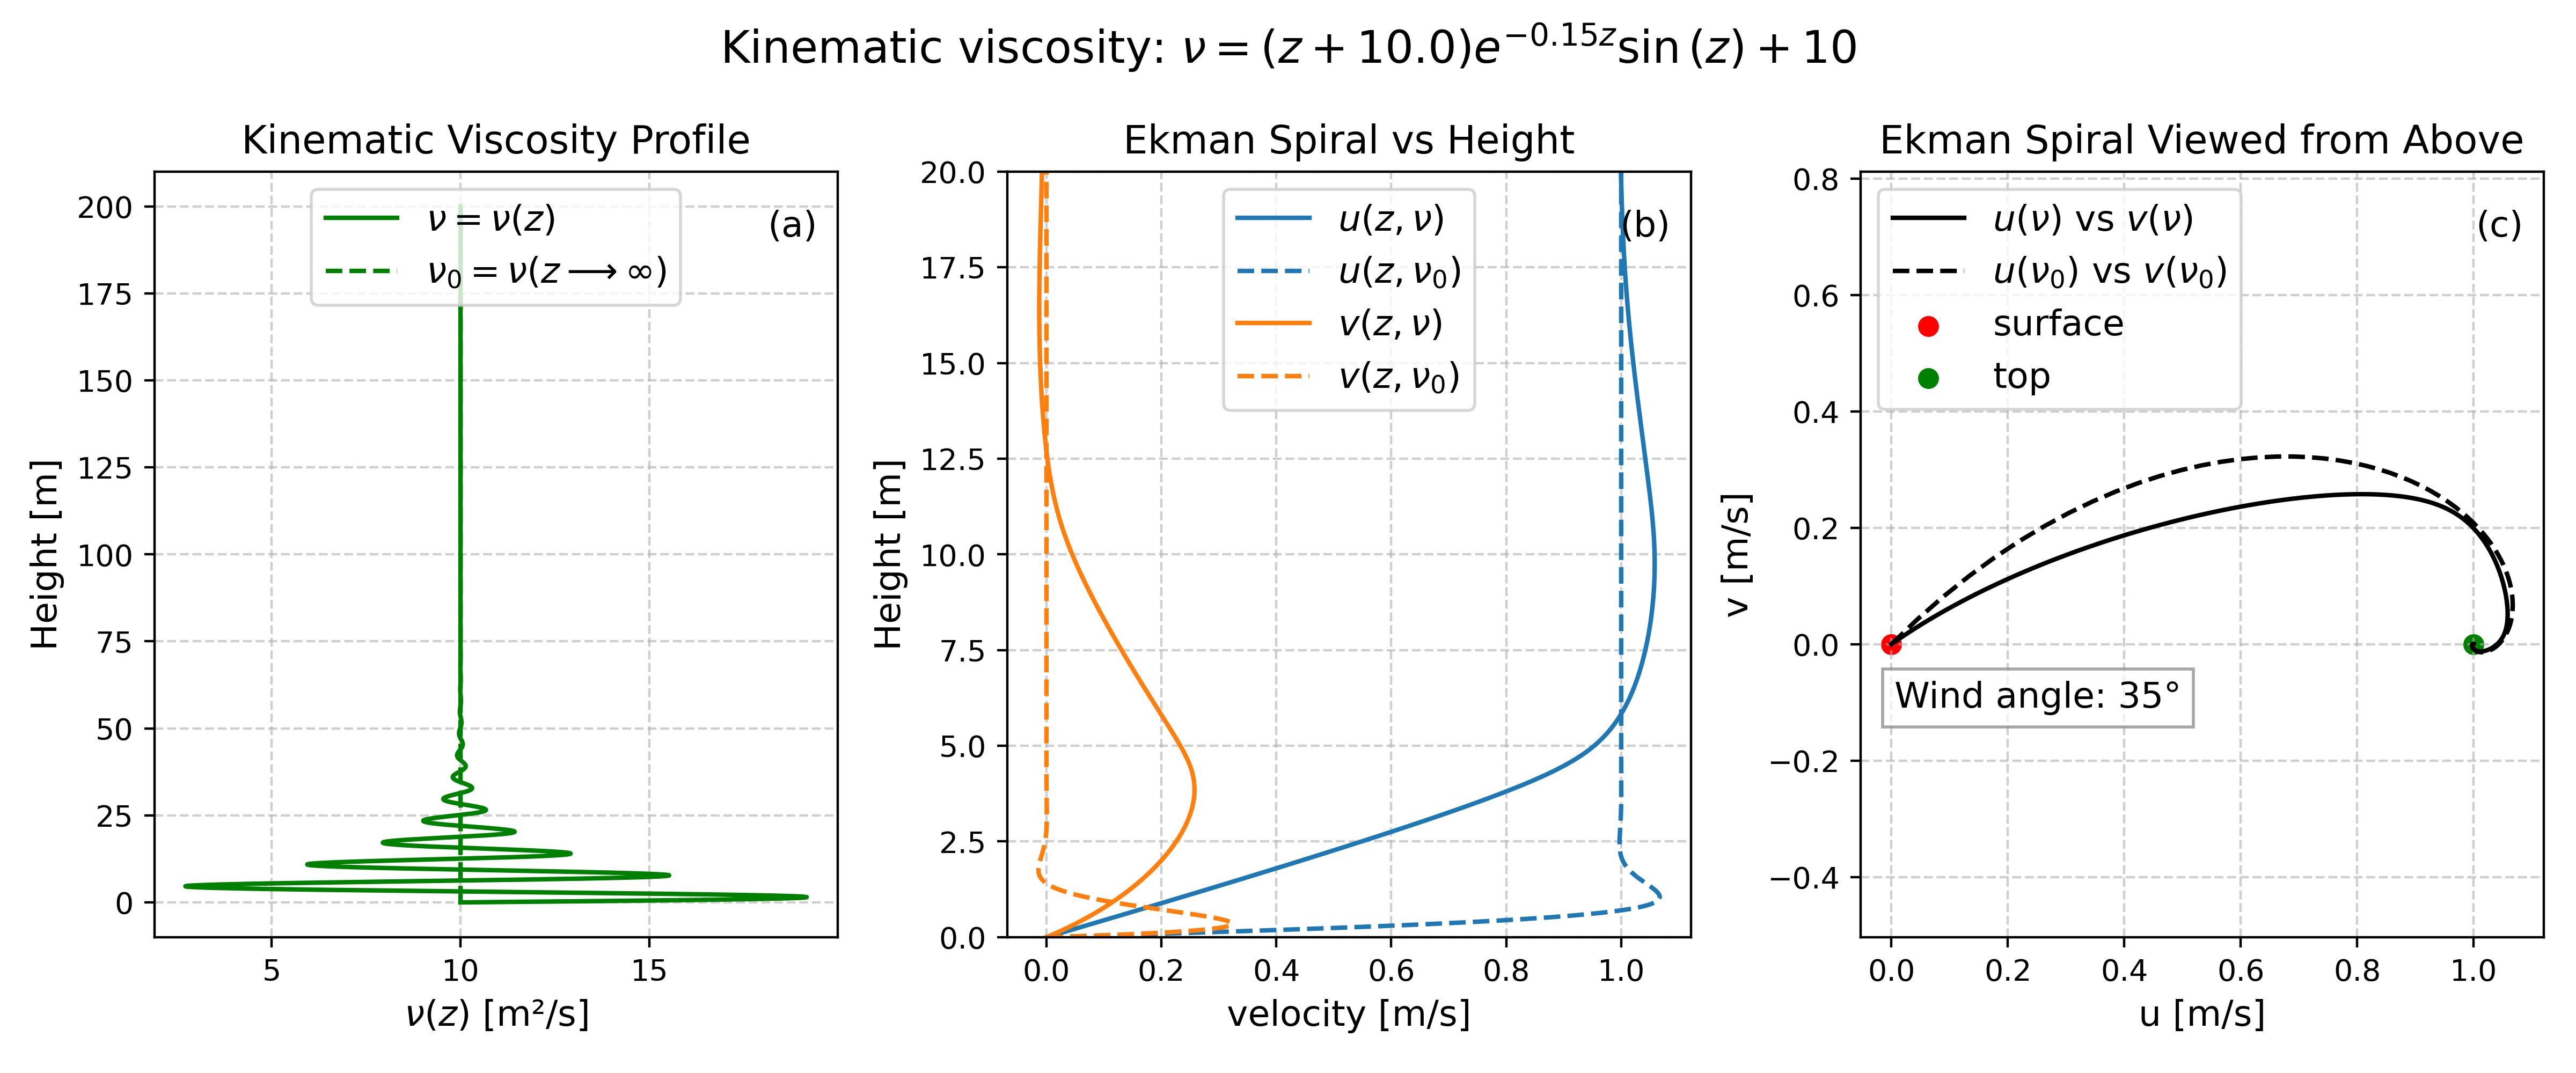
\includegraphics[width=0.9\textwidth]{Figures/BVP_fun.png}
    \caption{This figure shows the numeric solution for another specific profile.}
    \label{fig:numeric_fun}
\end{figure}

